\documentclass[12pt]{article} % Default font size is 12pt, it can be changed here
\usepackage[utf8]{inputenc}
\usepackage{geometry} % Required to change the page size to A4
\geometry{a4paper} % Set the page size to be A4 as opposed to the default US Letter
\usepackage{listings}
\usepackage{parskip}
\usepackage{xcolor}
\usepackage{float}
\usepackage{graphicx} % Required for including pictures
\usepackage{hyperref}
\usepackage{float} % Allows putting an [H] in \begin{figure} to specify the exact location of the figure
\usepackage{cite}
\usepackage{fancyhdr}

\linespread{1.2} % Line spacing

%\setlength{\parindent}{15pt}
%\setlength\parindent{0pt} % Uncomment to remove all indentation from paragraphs

\graphicspath{{../add/}} % Specifies the directory where pictures are stored

\pagestyle{fancy}
\lhead{Repositorio de árboles genealógicos en BD NoSQL}
\rhead{Daniel Albarral Nuñez}
\cfoot{\thepage}
\renewcommand{\headrulewidth}{0.4pt}
\renewcommand{\footrulewidth}{0.4pt}
\begin{document}

\begin{titlepage}

\newcommand{\HRule}{\rule{\linewidth}{0.5mm}} % Defines a new command for the horizontal lines, change thickness here

\center % Center everything on the page
 
%----------------------------------------------------------------------------------------
%	HEADING SECTIONS
%----------------------------------------------------------------------------------------

\textsc{\LARGE Universidad Politécnica de Cataluña}\\[1.5cm] % Name of your university/college
\textsc{\Large Facultad de Informática de Barcelona}\\[0.5cm] % Major heading such as course name
\textsc{\large Ingeniería de software}\\[0.5cm] % Minor heading such as course 

%----------------------------------------------------------------------------------------
%	TITLE SECTION
%----------------------------------------------------------------------------------------

\HRule \\[0.4cm]
{ \huge \bfseries Repositorio de árboles genealógicos en BD NoSQL}\\[0.4cm] % Title of your document
\HRule \\[1.5cm]
 
%----------------------------------------------------------------------------------------
%	AUTHOR SECTION
%----------------------------------------------------------------------------------------

\begin{minipage}{0.4\textwidth}
\begin{flushleft} \large
\emph{Author:}\\
Daniel \textsc{Albarral Nuñez} % Your name
\end{flushleft}
\end{minipage}
~
\begin{minipage}{0.4\textwidth}
\begin{flushright} \large
\emph{Supervisor:} \\
Enric \textsc{Mayol} % Supervisor's Name
\end{flushright}
\end{minipage}\\[4cm]

% If you don't want a supervisor, uncomment the two lines below and remove the section above
%\Large \emph{Author:}\\
%John \textsc{Smith}\\[3cm] % Your name

%----------------------------------------------------------------------------------------
%	DATE SECTION
%----------------------------------------------------------------------------------------

{\large Q1 - 2015-2016}\\[2cm] % Date, change the \today to a set date if you want to be precise

%----------------------------------------------------------------------------------------
%	LOGO SECTION
%----------------------------------------------------------------------------------------


\includegraphics[scale=0.7]{add/logo_upc.png}\\[1cm] % Include a department/university logo - this will require the graphicx package
 
%----------------------------------------------------------------------------------------

\vfill % Fill the rest of the page with whitespace

\end{titlepage}

%----------------------------------------------------------------------------------------
%   TABLE OF CONTENTS
%----------------------------------------------------------------------------------------

\tableofcontents % Include a table of contents

\newpage % Begins the essay on a new page instead of on the same page as the table of contents 


\section{Estado del arte}
Este proyecto se plantea como objeto de estudio y desarrollo la creación de un software orientado a que varios usuarios puedan gestionar arboles genealógicos. El software también ha de ser capaz de trabajar con la datos introducidos por los usuarios, para extraer información que pueda ser útil para ellos. Este tipo de software se llama software genealógico.

\subsection{Contextualización}

\subsubsection{Los arboles genealógicos}
Un arboles genealógico, también llamado genorama, es la representación gráfica de los antepasados  y descendientes de un individuo.Para su representación  se suelen usar tablas o arboles, siendo esta ultima la forma más común y la que se usara en el proyecto.

\subsubsection{Uso y aplicación de los arboles genealógicos}
Los arboles genealógicos son una herramienta de la genealogía, que se encarga de estudiar y seguir la ascendencia y descendencia de una persona o familia. La genealogía es una ciencia auxiliar de la Historia y es trabajada por un genealogista. Uno de los objetivos del software a desatollar es dar soporte a los genealogistas. \linebreak Por otro lado hay varias comunidades de aficionados que llevan sus propios arboles genealógicos, el software creado también les podrá dar servicio a esta tipología de usuarios.

\newpage
\subsection{Perspectiva general del software actual.}
Todo software genealógico, como mínimo permite almacenar la siguiente información de un individuo: fecha y lugar de nacimiento, fecha de casamiento, muerte y relaciones familiares, contra más flexible es el programa más información te permite introducir acerca de un individuo. También proporcionan diferentes maneras de representar la información y permiten exportar a GEDCOM la información representada.

\noindent\fbox{\parbox{\textwidth}{\begin{flushleft} GEDCOM \cite{aboutGEDCOM} (\textbf{G}enealogical \textbf{D}ata \textbf{COM}munication):\end{flushleft} Es un formato de archivo de datos, proporciona un formato flexible y uniforme para el intercambio de datos genealógicos computarizados.}}

La mayor parte del software genealógico actual esta basado en soluciones de escritorio, pero en los últimos años han aparecido diferentes soluciones web como myheritage o familysearch, que no solo sirven como plataforma de edición sino que también son grandes bases de datos.

Las soluciones más avanzadas en este ámbito aparte de la gestión de arboles también ofrecen herramientas más orientada a la investigación, como podrían ser sistemas de búsqueda de individuos basados en sus relaciones o herramientas estadística.

\subsection{Tecnología}
Dada la naturaleza social del tipo de software que se busca desarrollar, nacen ciertas complicaciones tecnológicas que en los últimos tiempos se han sido considerablemente investigadas, debido a la gran repercusión de las redes sociales. Las tecnologías clásicas orientadas a la persistencia de datos como las bases de datos SQL, plantean la dificultad de tener un coste muy alto de consulta cuando se pregunta acerca de datos  con un alto nivel de relación entre ellos. Una de las soluciones más usadas para solucionar este problema son las bases de datos basadas en grafos, uno de los casos de éxito es el caso de Twitter, que desarrollo su propia solución, FolckDB, una base de datos basada en grafos, tolerante a fallos, diseñada para tratar con grandes conjuntos de datos, con información no critica.

\subsubsection{Bases de datos basadas en grafos.}
La gran cantidad de proyectos que han nacido en los últimos años hace prácticamente imposible hacer una comparativa concreta de todas las tecnologías existentes. Pero podemos diferenciar el panorama actual haciendo dos generalizaciones:
\begin{description}
\item[Tecnologías usadas para propósitos transaccionales].\linebreak Orientadas ha dar un servicio online en tiempo real a una aplicación.
\linebreak Estas tecnologías son llamadas \textbf\textit{bases de datos basadas en grafos}. Estas son nuestro principal objeto de estudio. Son el equivalente a las OLTP en el modelo transaccional.
\item[Tecnologías usadas principalmente para el análisis de grafos].\linebreak Llamados \textbf\textit{Motores de procesamiento de grafos}, siguiendo el mismo símil que antes, podríamos pensarlos como herramientas de \textit{data mining} y análisis de procesos(OLAP)
\end{description}

\noindent\fbox{\parbox{\textwidth}{\begin{flushleft} OLTP (\textbf{O}n\textbf{L}ine \textbf{T}ransaction \textbf{P}rocessing):\end{flushleft} Es un tipo de procesamiento que facilita y administra aplicaciones transaccionales, usualmente para entrada de datos y recuperación y procesamiento de transacciones (gestor transaccional). Los paquetes de software para OLTP se basan en la arquitectura cliente-servidor ya que suelen ser utilizados por empresas con una red informática distribuida..}}

Las bases de datos basadas en grafos son sistemas de bases de datos que permiten operaciones CRUD (\textit{Create, Read, Update y Delete}) sobre los objetos representados en ellas. Suelen estar orientadas a funcionar con sistemas transaccionales (OLTP), como aviamos mencionado anteriormente. Sus principales propiedades son, las relaciones son \textit{ciudadanos de primer orden}, a diferencia de otros modelos, como el relacional que tienen que usar claves foráneas. En este tipo de base de datos para representar el dominio de nuestro problema simplemente nos basta con definir los nodos y las relaciones que lo componen.

En el libro Graph Databases \cite{graphdbbook}, encontramos el siguiente gráfico (Figure \ref{fig:grdb}), que nos da una idea de las principales tecnologías basadas en grafos y a que están más orientadas.

\begin{figure}[ht!]
\center
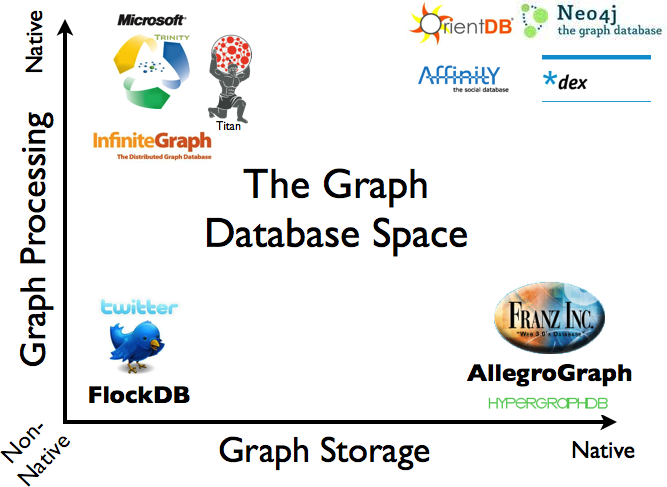
\includegraphics{add/grdb.png}
\caption{Visión del conjunto de tecnologías}
\label{fig:grdb}
\end{figure}

\section{Alcance} 
En este proyecto se desarrolla un software para la gestión y extracción de información de arboles genealógicos. El desarrollo de este software constara de dos fases principales que podemos asilar casi en su totalidad, el desarrollo de una plataforma web para la gestión de los arboles y un sistema que trabaje sobre los datos del sistema, con el objetivo de inferir información relevante del sistema de gestión. 

En lo referente a la plataforma web de gestión de arboles genealógicos, constara de un sistema de usuarios que permitirá que estos se conecten a la plataforma para gestionar y almacenar sus propios arboles genealógicos. Los usuarios podrán añadir otros usuarios a sus arboles genealógicos dándoles permiso de edición sobre estos y dando la opción de hacer los arboles públicos, las funcionales concretas se especificaran en las historias de usuario.
Este sistema se desarrollara maximizando el aislamiento ente sus componentes para favorecer su mantenibilidad y escalabilidad, con el objetivo de dejar un sistema abierto al desarrollo continuado. Para conseguir este objetivo se trabajara con metodologías ágiles y se dividirá el desarrollo en:
Especificación de un modelo conceptual y implantación en una base de datos basada en grafos (NoSQL) orientada a la optimización de consultas con un alto nivel de interdependencia entre objetos.
Una API que ofrezca las operaciones CRUD sobre la BD y gestione el sistema de usuarios y sus \textit{tokens} de acceso.
Un \textit{frontend} basado en tecnología web para que los usuarios hagan uso del sistema.

Por otro lado, el sistema encargado de inferir información estará compuesto por demonios que trabajaran usando la API del sistema de gestión. Dado que los objetos que componen la información  del sistema de gestión tiene una alta dependencia entre ellos, como ya se ha comentado anteriormente, los demonios tendrán que aprovechar al máximo las herramientas que proporciona la base de datos basada en grafos. La principal función de estos demonios sera encontrar coincidencias entre arboles genealógicos de diferentes usuarios.

\subsubsection{Posibles obstáculos}

\paragraph{Tiempo:}
La gestión del tiempo sera uno de los obstáculos más notables a la hora de desarrollar el proyecto, dado que se pretende plantear un proyecto que no necesariamente ha de concluir su desarrollo con la entrega final, para ello se tendrán que plantear claramente las iteraciones necesarias para tener una versión funcional del software y el tiempo de desarrollo que requerirán.
\paragraph{Integración de tecnologías y desarrollo:}
Uno de los objetivos de este proyecto es combinar ciertas tecnologías con las que no se ha trabajado anteriormente como bases de datos basadas en grafos y \textit{frameworks} JavaScrip para la implementación del \textit{frontend}. Por ello este hecho se tendrá que tener en cuenta en la planificación temporal.

\newpage
\subsubsection{Metodología}
El proyecto se desarrollara mediante una adaptación de Scrum que se adecue a las necesidades del proyecto.
Los roles se definirán de la siguiente forma:
\begin{description}
\item[\textit{product owner:}] El tutor de proyecto asumirá el rol de \textit{product owner} ya que sera el que definirá las historias de usuario y las priorizara.
\item[Equipo de desarrollo y Facilitador:] Dada la naturaleza del proyecto el equipo de desarrollo solo sera el alumno que a la vez ha de actuar como facilitador procurando que se cumplan los objetivos de los \textit{sprints}.
Por otro lado el \textit{product backlog} se definiría durante la asignatura de GEP.
\end{description}

\subsubsection{Herramientas de seguimiento}
Dado que el método de trabajo esta basado en Scrum, se usaran las estrategias de seguimiento establecidas por esta metodologías  de trabajo ágil.
En la fase de desarrollo se harán \textit{sprints} de dos semanas, al principio de cada \textit{sprint} se hará el \textit{Sprint planning} donde se escogerán que historias de usuarios serán desarrolladas. Al final del \textit{Sprint} se hará el \textit{sprint backlog} donde se revisara el trabajo realizado.

\newpage

\bibliography{mybibliography}
\nocite{*}
\bibliographystyle{plain}

\end{document}



